
%(BEGIN_QUESTION)
% Copyright 2014, Tony R. Kuphaldt, released under the Creative Commons Attribution License (v 1.0)
% This means you may do almost anything with this work of mine, so long as you give me proper credit

Hvis en {\it skilletransformator} (en transformator med samme antall ``vindinger'' i primær- og sekundærspolen) kobles mellom en AC-kilde og en AC-last, vil vi måle samme spenning og samme strøm ved både kilde- og lastterminalene:

$$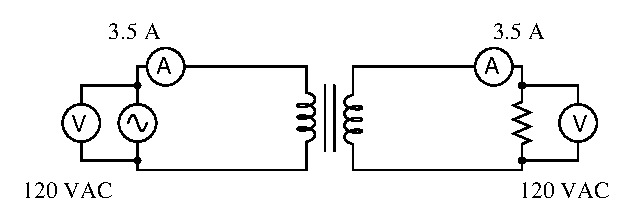
\includegraphics[width=15.5cm]{i01253x01.eps}$$

Hvis vi beregner effekten levert av kilden og effekten avsatt i lasten, er verdien den samme: 420 Watt ($P = IV$).

\vskip 10pt

Anta nå at vi analyserer en krets som inneholder en {\it opptransformator} (en med flere vindinger i sekundærspolen enn i primærspolen). Med en opptransformator vil lastspenningen være større enn forsyningsspenningen. I dette eksempelet viser jeg en opptransformator med et 1:2 omsetningsforhold:

$$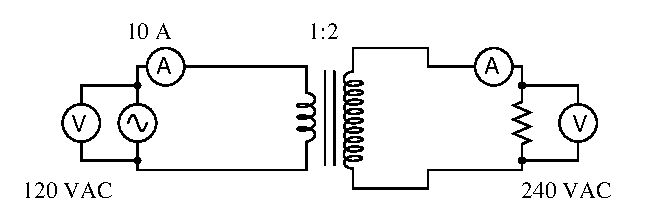
\includegraphics[width=15.5cm]{i01253x02.eps}$$

Anta at lastmotstanden er helt forskjellig fra den første (skilletransformator) kretsen. Hva kan du utlede om laststrømmen og effekten (både kilde og last) i denne kretsen? Er laststrømmen mindre enn kildestrømmen? Er laststrømmen større enn kildestrømmen? Er lasteffekten større enn kildeeffekten? Forklar svarene dine.

\underbar{file i01253}
%(END_QUESTION)





%(BEGIN_ANSWER)

Den grunnleggende fysiske loven kjent som {\it Loven om energibevaring} forteller oss at energi ikke kan komme fra intet, eller forsvinne i intet. Hvis strømkilden sender 420 watt inn i transformatoren, må lasten motta 420 watt (hvis vi ser bort fra eventuelle interne ineffektiviteter i transformatoren). Transformatorens omsetningsforhold er helt irrelevant når det gjelder {\it effekt}!

\vskip 10pt

For en reell transformator (med mindre enn 100\% virkningsgrad), vil lasten motta litt mindre enn 420 watt effekt, og resten omdannes til varme i transformatoren.

%(END_ANSWER)





%(BEGIN_NOTES)

Den eneste grunnen til at jeg nøler med å fortelle studentene at de kan beregne laststrømmen {\it nøyaktig}, er at det ikke ble oppgitt om transformatoren har ``tap'' i det hele tatt. Ingen reell transformator er 100\% tapsfri, selvfølgelig, og dette er noe vi må ta i betraktning i ``det virkelige liv''.

Jeg har funnet ut at tilnærmingen med energibevaring ikke bare gir mening for studentene når de lærer å beregne transformatoroppførsel, men det er også en utmerket forsterkning av en grunnleggende fysisk lov, som vil tjene dem godt gjennom hele karrieren hvis de forstår den godt.

%INDEX% Electronics review: transformer ratios

%(END_NOTES)
